% TIKZ BEAMER
\documentclass[12pt]{article}
\usepackage[utf8]{vietnam}
% Căn lề
\usepackage[left=3.5cm, right=2cm,
top=2cm, bottom=2cm]{geometry}
% Các gói toán học
\usepackage{amsmath}
\usepackage{amssymb}
\usepackage{amsthm}
% Gói hình ảnh
\usepackage{graphicx}
% Khai báo thư viện Tikz
% usetikzlibrary{(tikz library)}
\usepackage{tikz}

\begin{document}
% Tham số cần thiết
% Độ rộng nét vẽ ultra thin, very thin, semithick, very thick, ultra thick,,... 
% Nét đứt: dashed, dotted

% Thiết lập style cho tikzstyle
\tikzstyle{mystyle} = [red,thick,dashed,->]
% Môi trường tikz
% + tham số every picture
\begin{tikzpicture}
	% Vẽ lưới toạ độ ô vuông 
	% Đơn vị đo là 1 ô cm^2
	\draw [help lines] (-3,-3)  grid (5,5);
	\draw [red,thick,dashed] (0,0)--(4,4);
	\draw [mystyle] (0,0)--(-4,4);
	
	\coordinate[label=A] (A) at (0,0);
	
	\draw[xshift=1cm,blue] (0,0)--++(1,0)--++(0,1);
	\draw[xshift=3cm,blue] (0,0)--+(1,0)--+(0,1);

	\node[below left] at (0,-3) {(0)};
	\node[below left] at (A) {(0,0)};
	\fill[red,opacity=0.5] (0,0)--(0,1)--(1,1)--(1,0)--cycle;
	\filldraw[xshift=2cm,blue,opacity=0.5] (0,0)--(0,1)--(1,1)--(1,0)--cycle;
\end{tikzpicture}

% Path
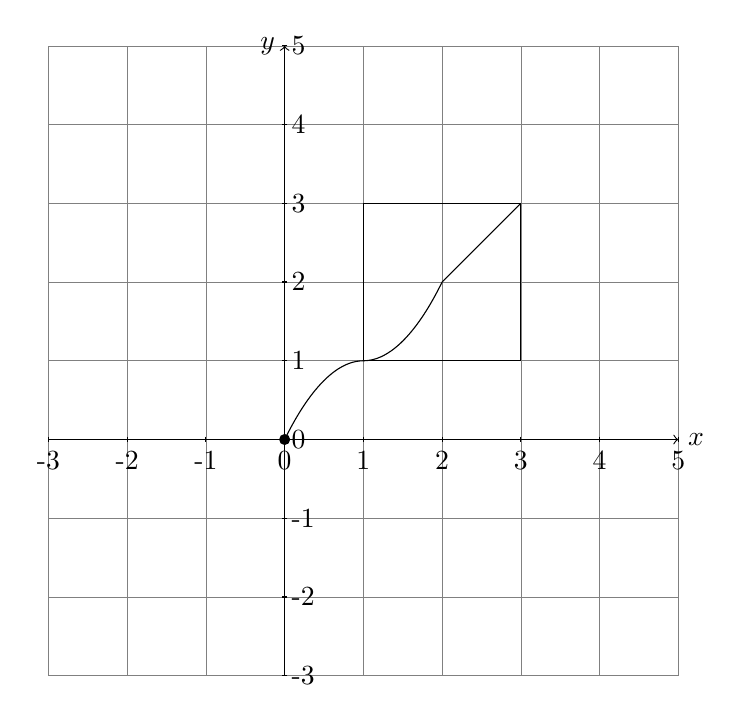
\begin{tikzpicture}
	\draw [help lines] (-3,-3)  grid (5,5);
	\fill (0,0) circle (2pt);
	\draw[->] (-3,0)--(5,0) node [right] {$x$};
	\draw[->] (0,-3)--(0,5) node [left] {$y$};
	\foreach \x in {-3,-2,...,5}
	{
	\draw (\x,1pt)--(\x,-1pt) node [below] {\x};
	\draw (1pt,\x)--(-1pt,\x) node [right] {\x};
	}
	\draw (2,2)--(3,3);
	\draw (1,1)-|(3,3);
	\draw (1,1)|-(3,3);
	\draw (0,0) parabola bend (1,1) (2,2);
\end{tikzpicture}

% Function
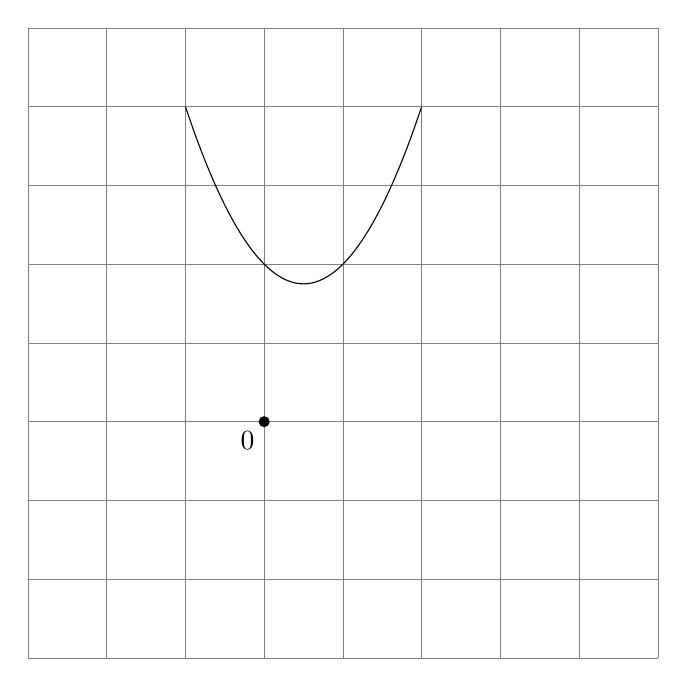
\begin{tikzpicture}
	\draw [help lines] (-3,-3)  grid (5,5);
	\fill (0,0) circle (2pt);
	\node (0,0) [below left] {0};
	% draw function
	\draw [domain=-1:2,samples=25,smooth] plot (\x,{(\x)^2-(\x)+2});
\end{tikzpicture}
\end{document}